\appendix
\section{Random Latent Exploration}

\noindent The architecture of our RLE implementation can be found in figure \ref{fig:rle-architecture}:

\begin{figure}[h!]
  \centering
  %\includegraphics[width=0.5\textwidth]{tikz/rle-architecture.tex}
  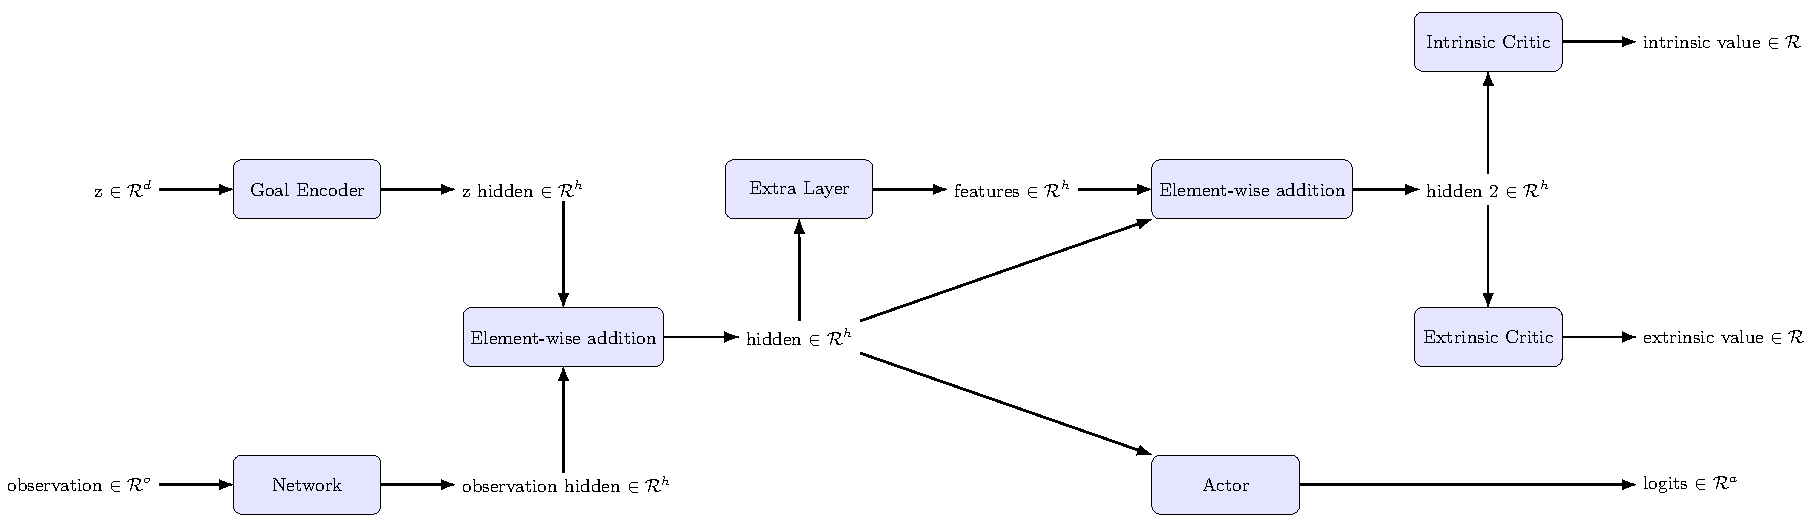
\includegraphics[width=\textwidth]{tikz/rle-architecture-modified.tex}
  \caption{In RLE, the policy and critic networks are conditioned on the latent vector z. \cite{rle-paper} split the critic's head in two: one head predicts the extrinsic value and the other head predicts the intrinsic value. In the vector dimension, $o$ represents the dimension of a single observation, $d$ represents the RLE feature dimension, and $a$ is the cardinality of the action space.}
  \label{fig:rle-architecture}
\end{figure}

\noindent For the RLE algorithm, the detailed pseudocode according to \cite{rle-paper} is as follows:

\hypertarget{algo-rle}{
\begin{table}[h!]
  \centering
  \begin{tabular}{rlllll}
    \hline\hline
    \textbf{RLE:} & \multicolumn{5}{l}{Detailed Pseudocode}\\
    \hline
    1: & \multicolumn{5}{l}{\textbf{Input:} Latent distribution $\left(P_{\textbf{z}}\right)$, number of parallel workers $\left(N\right)$, number of steps per update}\\
    & \multicolumn{5}{l}{$\left(T\right)$, number of steps per sampling $\left(S\right)$, and feature network update rate $\left(\tau\right)$.}\\
    2: & \multicolumn{5}{l}{Randomly initialize a feature network $\left(\phi\right)$ with the same backbone architecture as the policy }\\
    & \multicolumn{5}{l}{and value networks.}\\
    3: & \multicolumn{5}{l}{Initialize running mean $\boldsymbol{\mu} = \textbf{0}$ and standard deviation $\boldsymbol{\sigma} = \textbf{1}$ estimates of $\boldsymbol{\phi} \left(s\right)$ over the state}\\
    & \multicolumn{5}{l}{space.}\\
    4: & \multicolumn{5}{l}{Sample an initial latent vector $\textbf{z} \sim P_{\textbf{z}}$ for each parallel worker.}\\
    5: & \multicolumn{5}{l}{\textbf{Repeat (\textsuperscript{1})}}\\
    6: & | & \multicolumn{4}{l}{Sample initial state $s_{0}$.}\\
    7: & | & \multicolumn{4}{l}{\textbf{For} $t = 0, ..., T$ \textbf{do (\textsuperscript{2})}}\\
    8: & | & | & \multicolumn{3}{l}{Take action $a_{t} \sim \boldsymbol{\pi}(. | s_{t}, \textbf{z})$ and transition to $s_{t+1}$.}\\
    9: & | & | & \multicolumn{3}{l}{Compute feature $\textbf{f}(s_{t+1}) = \frac{\boldsymbol{\phi}(s_{t+1}) - \boldsymbol{\mu}}{\boldsymbol{\sigma}}$.}\\
    10: & | & | & \multicolumn{3}{l}{Compute random reward $F(s_{t+1}, \textbf{z}) = \frac{\textbf{f}(s_{t+1})}{\| \textbf{f}(s_{t+1}) \|} \cdot \textbf{z}$.}\\
    11: & | & | & \multicolumn{3}{l}{Receive reward $r_{t} = R(s_{t}, a_{t}) + F(s_{t+1}, \textbf{z})$.}\\
    12: & | & | & \multicolumn{3}{l}{\textbf{For} $i = 0, 1, ..., N-1$ \textbf{do (\textsuperscript{3})}}\\
    13: & | & | & | & \multicolumn{2}{l}{\textbf{If} worker $i$ terminated \textbf{or} $S$ timesteps passed without resampling, \textbf{then (\textsuperscript{4})}}\\
    14: & | & | & | & | & Resample sample $\textbf{z} \sim P_{\textbf{z}}$ for worker $i$.\\
    15: & | & | & | & \multicolumn{2}{l}{\textbf{(\textsuperscript{4})}}\\
    16: & | & | & \multicolumn{3}{l}{\textbf{(\textsuperscript{3})}}\\
    17: & | & \multicolumn{4}{l}{\textbf{(\textsuperscript{2})}}\\
    18: & | & \multicolumn{4}{l}{Update policy network $\boldsymbol{\pi}$ and value network $V_{\boldsymbol{\pi}}$ with the collected trajectory}\\
    & | & \multicolumn{4}{l}{$(\textbf{z}, s_{0}, a_{0}, r_{0}, s_{1}, ..., s_{T})$.}\\
    19: & | & \multicolumn{4}{l}{Update feature network $\boldsymbol{\phi}$ using the value network's parameters $\boldsymbol{\phi} \leftarrow \tau \cdot V^{\boldsymbol{\pi}} + (1 - \tau) \cdot \boldsymbol{\phi}$.}\\
    20: & | & \multicolumn{4}{l}{Update $\boldsymbol{\mu}$ and $\boldsymbol{\sigma}$ using the batch of collected experience.}\\
    21: & \multicolumn{5}{l}{\textbf{(\textsuperscript{1}) until convergence}}\\
    \hline\hline
  \end{tabular}
\end{table}}

\clearpage
\hypertarget{algo-ppo}{\section{Proximal Policy Optimization}}

\noindent The algorithm constituting the foundation of RLE is Proximal Policy Iteration (PPO), described in \cite{ppo-paper}, which can itself be run to solve RL problems. It is an on-line policy gradient method where after running the policy $\boldsymbol{\pi}_{\theta_{\text{old}}}$ in parallel with $N$ actors for $T << E$ timesteps, where $E$ is the length of an episode, we compute the advantage estimator as proposed by \cite{generalized-advantage-estimation-paper} for each time index $t \in [0, T]$:

\begin{equation}
  \hat{A}_{t} = \delta_{t} + \left(\gamma \lambda\right) \delta_{t+1} + ... + \left(\gamma \lambda\right)^{T-t+1} \delta_{T - 1}
  \label{eq:ppo-advantage-estimator}
\end{equation}

\noindent where we have $\delta_{t} = r_{t} + \gamma V(s_{t+1}) - V(s_{t})$. Here, $\lambda$ is the Generalized Advantage Estimation (GAE) parameter and $V(s)$ is a learned state-value function. Afterwards, for each $t$ the surrogate objective is computed and the parameters $\theta$ are optimized e.g. with minibatch SGD or Adam (note that we optimize by maximizing the objective). This surrogate objective takes the form:

\begin{equation}
  L_{t}^{\text{CLIP} + \text{VF} + \text{S}}(\theta) = \hat{\mathbb{E}}_{t} \left[L_{t}^{\text{CLIP}}(\theta) - c_{1} L_{t}^{\text{VF}}(\theta) + c_{2} S[\boldsymbol{\pi}_{\theta}](s_{t})\right]
  \label{eq:ppo-objective-function}
\end{equation}

\noindent In \eqref{eq:ppo-objective-function}, we have the VF coefficient $c_{1}$ and the entropy coefficient $c_{2}$, together with the (optional, to enhance exploration) entropy bonus $S[\boldsymbol{\pi}_{\theta}](s_{t})$, which is calculated as the sum of $- p \log{p}$ over each of the action-probabilities $p$ resulting from the policy distribution $\boldsymbol{\pi}_{\theta}$ for a state $s_{t}$, and the objectives:

\begin{align}
  \label{eq:ppo-clip-objective} L_{t}^{\text{CLIP}}(\theta) &= \hat{\mathbb{E}}_{t}\left[\min\left(r_{t}(\theta) \hat{A}_{t}, \text{clip}\left(r_{t}(\theta), 1 - \epsilon, 1 + \epsilon\right) \hat{A}_{t}\right)\right]\\
  \label{eq:ppo-vf-objective} L_{t}^{\text{VF}}(\theta) &= \left(V_{\theta}(s_{t}) - V_{t}^{\text{targ}}\right)^{2}
\end{align}

\noindent In \eqref{eq:ppo-clip-objective} we denote the probability ratio as $r_{t}(\theta) = \frac{\pi_{\theta}\left(a_{t}|s_{t}\right)}{\pi_{\theta_{\text{old}}}(a_{t}|s_{t})}$, where $\pi_{\theta_{\text{old}}}$ is the policy before the update, and the clipping function is:

\begin{equation}
  \text{clip}\left(r_{t}(\theta), 1 - \epsilon, 1 + \epsilon\right) = \begin{cases}
    1 - \epsilon, &r_{t}(\theta) < 1 - \epsilon\\
    r_{t}(\theta), &1 - \epsilon \leq r_{t}(\theta) \leq 1 + \epsilon\\
    1 + \epsilon, &r_{t}(\theta) > 1 + \epsilon
  \end{cases}
  \label{eq:clipping-function}
\end{equation}

\noindent Moreover in \eqref{eq:ppo-vf-objective}, $V_{t}^{\text{targ}}$ represents some target state-value function that is to be obtained. Note that there exist also other objective functions mentioned in \cite{ppo-paper} that can substitute $L_{t}^{\text{CLIP}}(\theta)$ in \eqref{eq:ppo-objective-function}. In \eqref{eq:clipping-function}, we make use of a hyperparameter $\epsilon \in [0, 1]$ and in combination with the minimizer from \eqref{eq:ppo-clip-objective} we can prevent a single policy update to accidentally ruin the policy forever by sending the algorithm to a gradient region with a worse local extremum.

\noindent For the PPO algorithm, the detailed pseudocode according to \cite{ppo-paper} is as follows:

\begin{table}[h!]
  \centering
  \begin{tabular}{rlll}
    \hline\hline
    \textbf{PPO:} & \multicolumn{3}{l}{Detailed Pseudocode, Actor-Critic Setup}\\
    \hline
    1: & \multicolumn{3}{l}{\textbf{Input:} Number of iterations $\left(I\right)$, number of actors $\left(N\right)$, number of timesteps per iteration}\\
    & \multicolumn{3}{l}{$\left(T\right)$, number of epochs $(K)$, minibatch size $(M \leq NT)$, learned state-value function implicitly}\\
    & \multicolumn{3}{l}{in the advantage estimator $(V(s))$, target value $(V_{t}^{\text{targ}})$ implicitly in the objective $L$.}\\
    2: & \multicolumn{3}{l}{\textbf{For} $i = 1, ..., I$ \textbf{do (\textsuperscript{1})}}\\
    3: & | & \multicolumn{2}{l}{\textbf{For} $n = 1, ..., N$ \textbf{do (\textsuperscript{2})}}\\
    4: & | & | & Run policy $\boldsymbol{\pi}_{\theta_{\text{old}}}$ in environment for $T$ timesteps.\\
    5: & | & | & Compute advantage estimates $\hat{A}_{1}, ..., \hat{A}_{T}$.\\
    6: & | & \multicolumn{2}{l}{\textbf{(\textsuperscript{2})}}\\
    7: & | & \multicolumn{2}{l}{Optimize objective $L$ w.r.t. $\theta$, for given $K$ and $M$, using e.g. minibatch SGD or Adam.}\\
    8: & | & \multicolumn{2}{l}{Update parameters $\theta_{\text{old}} \leftarrow \theta$.}\\
    9: & \multicolumn{3}{l}{\textbf{(\textsuperscript{1})}}\\
    \hline\hline
  \end{tabular}
\end{table}

\clearpage
\hypertarget{algo-noisynet}{\section{NoisyNet}}

\noindent The central idea in a NoisyNet architecture brought forward by \cite{noisynet-paper} is to introduce random noise into the weights learned by the network ($p$ inputs, $q$ outputs), i.e. if we have a neural network whose output can be parametrized by a vector of weights $\boldsymbol{\theta}$ as $\textbf{y} = f_{\boldsymbol{\theta}}(\textbf{x}) = \textbf{w} \cdot \textbf{x} + \textbf{b}$, then we can learn the set of parameter vectors $\zeta = (\boldsymbol{\mu}, \boldsymbol{\Sigma})$ to compute $\textbf{w} = (\boldsymbol{\mu}^{w} + \boldsymbol{\sigma}^{w} \odot \boldsymbol{\varepsilon}^{w})$ and $\textbf{b} = (\boldsymbol{\mu}^{b} + \boldsymbol{\sigma}^{b} \odot \boldsymbol{\varepsilon}^{b})$ with the following dimensionalities: $\boldsymbol{\mu}^{w}$, $\boldsymbol{\sigma}^{w}$, $\boldsymbol{\varepsilon}^{w} \in \mathbb{R}^{q \times p}$ implying $\textbf{w} \in \mathbb{R}^{q \times p}$, and $\boldsymbol{\mu}^{b}$, $\boldsymbol{\sigma}^{b}$, $\boldsymbol{\varepsilon}^{b} \in \mathbb{R}^{q}$ resulting in $\textbf{b} \in \mathbb{R}^{q}$. Note that $\textbf{x} \in \mathbb{R}^{p}$, $\textbf{y} \in \mathbb{R}^{q}$ and $\odot$ denotes element-wise multiplication.

\noindent We optimize the loss $\bar{L}(\zeta) = \mathbb{E}_{\varepsilon}[L(\boldsymbol{\theta})]$, i.e. the expectation of the loss $L(\boldsymbol{\theta})$ over the noise $\varepsilon$ which has a mean of zero and fixed statistics, using gradient descent on the parameters $\zeta$. The noise can be sampled either independently or in a factorized way from a Gaussian. The former method samples the noise $\varepsilon^{w}_{i,j} \in \boldsymbol{\varepsilon}^{w}$ and $\varepsilon^{b}_{j} \in \boldsymbol{\varepsilon}^{b}$ for every input to the network leading to a total of $pq + q$ random samples. Factorized sampling on the other hand greatly reduces computational complexity by factorizing $\varepsilon^{w}_{i,j} = f(\varepsilon_{i}) f(\varepsilon_{j})$ and then $\varepsilon^{b}_{j} = f(\varepsilon_{j})$ thereby lowering the number of required random samples to $p + q$, where $f: \mathbb{R} \rightarrow \mathbb{R}$. In \cite{noisynet-paper} the function $f(x) = \sign(x) \sqrt{|x|}$ is used. After sampling the noise, in theory we compute the gradients $\nabla\bar{L}(\zeta) = \nabla\mathbb{E}_{\varepsilon}[L(\boldsymbol{\theta})] = \mathbb{E}_{\varepsilon}[\nabla_{\boldsymbol{\mu}, \boldsymbol{\Sigma}}L(\boldsymbol{\mu} + \boldsymbol{\Sigma} \odot \boldsymbol{\varepsilon})]$, whereas in practice we approximate $\nabla\bar{L}(\zeta) \approx \nabla_{\boldsymbol{\mu}, \boldsymbol{\Sigma}}L(\boldsymbol{\mu} + \boldsymbol{\Sigma} \odot \boldsymbol{\varepsilon})$ with the Monte Carlo method.

\noindent In the code of \cite{rle-paper}, a NoisyNet is used in conjunction with the A3C-algorithm, in particular the loss is computed from the action-value function is estimated using:

\begin{equation}
  \hat{Q}_{i} = \sum_{j=i}^{k-1} \gamma^{j-i} r_{t+j} + \gamma^{k-i} V(x_{t+k} | \zeta, \varepsilon_{i})
\end{equation}

Moreover, for factorized networks, we initialize $\mu_{i,j} \sim \mathcal{U}\left[-\frac{1}{\sqrt{p}}, +\frac{1}{\sqrt{p}}\right]$ and $\sigma_{i,j} = \frac{\sigma_{0}}{\sqrt{p}}$ with $p$ being the number of inputs to the corresponding linear layer, $\mathcal{U}$ is a uniform distribution over the specified interval, and $\sigma_{0}$ is a hyperparameter.

\textcolor{red}{Are we using independent or factorized sampling in the code? (I'm guessing factorized).}

\noindent For the NoisyNet + A3C algorithm, the detailed pseudocode according to \cite{noisynet-paper} is as follows:

\begin{table}[h!]
  \centering
  \begin{tabular}{rlll}
    \hline\hline
    \textbf{NoisyNet:} & \multicolumn{3}{l}{Detailed Pseudocode, for each actor-learner thread}\\
    \hline
    1: & \multicolumn{3}{l}{\textbf{Input:} Global shared parameters $(\zeta_{\pi}, \zeta_{V})$, global shared counter $(T)$, and maximal}\\
    & \multicolumn{3}{l}{time $(T_{\text{max}})$.}\\
    2: & \multicolumn{3}{l}{\textbf{Input (each thread):} Thread-specific parameters $(\zeta_{\pi}', \zeta_{V}')$, set of random variables $(\varepsilon)$,}\\
    & \multicolumn{3}{l}{thread-specific counter $(t)$, and roll-out size $(t_{\text{max}})$.}\\
    3: & \multicolumn{3}{l}{\textbf{Output:} Policy $\pi(\cdot|\zeta_{\pi}, \varepsilon)$ and value function $V(\cdot|\zeta_{V},\varepsilon)$.}\\
    4: & \multicolumn{3}{l}{$t \leftarrow 1$}\\
    5: & \multicolumn{3}{l}{\textbf{Repeat (\textsuperscript{1})}}\\
    6: & | & \multicolumn{2}{l}{Reset cumulative gradients: $d\zeta_{\pi} \leftarrow 0, d\zeta_{V} \leftarrow 0$.}\\
    7: & | & \multicolumn{2}{l}{Synchronize thread-specific parameters: $\zeta_{\pi}' \leftarrow \zeta_{\pi}, \zeta_{V}' \leftarrow \zeta_{V}$.}\\
    8: & | & \multicolumn{2}{l}{Set counter $c \leftarrow 0$.}\\
    9: & | & \multicolumn{2}{l}{Get state $x_{t}$ from environment.}\\
    10: & | & \multicolumn{2}{l}{Sample noise $\xi \sim \varepsilon$.}\\
    11: & | & \multicolumn{2}{l}{Create lists for rewards $r \leftarrow [ ]$, actions $a \leftarrow [ ]$ and states $x \leftarrow [ ]$.}\\
    12: & | & \multicolumn{2}{l}{\textbf{Repeat (\textsuperscript{2})}}\\
    13: & | & | & Choose action $a_{t} \leftarrow \pi(\cdot|x_{t}, \zeta_{pi}', \zeta_{V}')$.\\
    14: & | & | & $a[-1] \leftarrow a_{t}$\\
    15: & | & | & Obtain reward $r_{t}$ and new state $x_{t+1}$.\\
    16: & | & | & $r[-1] \leftarrow r_{t}$, $x[-1] \leftarrow x_{t}$, $t \leftarrow t + 1$, $T \leftarrow T + 1$, $c \leftarrow c + 1$\\
    17: & | & \multicolumn{2}{l}{\textbf{(\textsuperscript{2}) until} $x_{t}$ \textbf{is terminal or} $c > t_{\text{max}}$}\\
    18: & | & \multicolumn{2}{l}{\textbf{If} $x_{t}$ is terminal, \textbf{then (\textsuperscript{3})}}\\
    19: & | & | & $Q \leftarrow 0$\\
    20: & | & \multicolumn{2}{l}{\textbf{else}}\\
    21: & | & | & $Q \leftarrow V\left(x_{t}|\zeta_{V}', \xi\right)$\\
    22: & | & \multicolumn{2}{l}{\textbf{(\textsuperscript{3})}}\\
    23: & | & \multicolumn{2}{l}{\textbf{For} $i = c - 1, ..., 0$ \textbf{do (\textsuperscript{4})}}\\
    24: & | & | & $Q \leftarrow r\left[i\right] + \gamma Q$\\
    25: & | & | & $d\zeta_{\pi} \leftarrow d\zeta_{\pi} \nabla_{\zeta_{\pi}'} \log{(\pi(a[i]|x[i], \zeta_{\pi}', \xi)) [Q - V(x[i]|\zeta_{V}', \xi)]}$\\
    26: & | & | & $d\zeta_{V} \leftarrow d\zeta_{V} \nabla_{\zeta_{V}'} \left[Q - V\left(x[i]|\zeta_{V}', \xi\right)\right]^{2}$\\
    27: & | & \multicolumn{2}{l}{\textbf{(\textsuperscript{4})}}\\
    28: & | & \multicolumn{2}{l}{Update asynchronously parameter $\zeta_{\pi} \leftarrow \zeta_{\pi} + \alpha_{\pi}d\zeta_{\pi}$.}\\
    29: & | & \multicolumn{2}{l}{Update asynchronously parameter $\zeta_{V} \leftarrow \zeta_{V} - \alpha_{V}d\zeta_{V}$.}\\
    30: & \multicolumn{3}{l}{\textbf{(\textsuperscript{1}) until} $T > T_{\text{max}}$}\\
    \hline\hline
  \end{tabular}
\end{table}

\hypertarget{algo-rnd}{\section{Random Network Distillation}}

In Random Network Distillation, as described by \cite{rnd-paper}, we compose the reward which the agent obtains as $r_{t} = e_{t} + i_{t}$ where $e_{t}$ represents a sparse extrinsic (environment's) reward and $i_{t}$ is the intrinsic reward for transitioning, i.e. the exploration bonus emanating from the transition at time step $t$. The latter measures the novelty of a state and should yield a higher value, the less frequently a state has been visited so far. In case of a finite state space we can use $i_{t} = \frac{1}{n_{t}}$ or $i_{t} = \frac{1}{\sqrt{s}}$ where $n_{t}(s)$ denotes the number of times state $s$ has been visited until time step $t$. However, there exist alternatives, e.g. we could use state density based approaches to calculate an exploration bonus, which are described in the paper mentioned above. Moreover, they specify that in the paper the intrinsic reward is the prediction error of a randomly generated problem $i_{t} = \|\hat{f}(x|\theta) - f(x)\|^{2}$ involving a target network $f: \mathcal{O} \rightarrow \mathbb{R}^{k}$ (fixed and randomly initialized, maps an observation $\mathcal{O}$ to an embedding $\mathbb{R}^{k}$) to sample the problem as well as a predictor network $\hat{f}: \mathcal{O} \rightarrow \mathbb{R}^{k}$ which was trained on the agent's data by gradient descent to optimize $i_{t}$ w.r.t. parameters $\theta_{\hat{f}}$.

\noindent Since the overall return can be composed as a sum of returns $R = R_{E} + R_{I}$ we can train two heads $V_{E}$ and $V_{I}$ to estimate the value function $V = V_{E} + V_{I}$ and in extension the advantages. In the end, a policy is trained with standard PPO using the advantage estimators. Note that the intrinsic rewards have to be normalized in order to be useful because otherwise we could not guarantee that they are on a consistent scale, which is done by dividing $i_{t}$ by a running estimate of the standard deviations of the intrinsic return. Furthermore, the observation also has to be normalized as $x \leftarrow \text{clip}(\frac{x - \mu}{\sigma}, -5, 5)$. The normalization parameters can be initialized by letting a random agent briefly move in the environment before beginning the optimization.

\noindent The detailed pseudocode according to \cite{rnd-paper} is as follows:

\begin{table}[h!]
  \centering
  \begin{tabular}{rlll}
    \hline\hline
    \textbf{RND:} & \multicolumn{3}{l}{Detailed Pseudocode}\\
    \hline
    1: & \multicolumn{3}{l}{\textbf{Input:} Number of rollouts $(N)$, Number of optimization steps $(N_{\text{opt}})$, and length of initial}\\
    & \multicolumn{3}{l}{steps for initializing observation normalization $(M)$.}\\
    2: & \multicolumn{3}{l}{$t \leftarrow 0$}\\
    3: & \multicolumn{3}{l}{Sample state $s_{0} \sim p_{0}(s_{0})$.}\\
    4: & \multicolumn{3}{l}{\textbf{For} $m = 1, ..., M$ \textbf{do (\textsuperscript{1})}}\\
    5: & | & \multicolumn{2}{l}{Sample action $a_{t} \sim \mathcal{U}(a_{t})$. \textcolor{red}{Are we sampling uniformly from all available actions at time $t$?}}\\
    6: & | & \multicolumn{2}{l}{Sample state $s_{t+1} \sim p(s_{t+1}|s_{t}, a_{t})$.}\\
    7: & | & \multicolumn{2}{l}{Update observation normalization parameters using $s_{t+1}$.}\\
    8: & | & \multicolumn{2}{l}{$t \leftarrow t + 1$}\\
    9: & \multicolumn{3}{l}{\textbf{(\textsuperscript{1})}}\\
    10: & \multicolumn{3}{l}{\textbf{For} $i = 1, ..., N$ \textbf{do (\textsuperscript{2})}}\\
    11: & | & \multicolumn{2}{l}{\textbf{For} $j = 1, ..., K$ \textbf{do (\textsuperscript{3})}}\\
    12: & | & | & Sample action $a_{t} \sim \pi(a_{t}|s_{t})$.\\
    13: & | & | & Sample state $s_{t+1}, e_{t} \sim p(s_{t+1}, e_{t}|s_{t}, a_{t})$.\\
    14: & | & | & Calculate intrinsic reward $i_{t} = \|\hat{f}(s_{t+1}) - f(s_{t+1})\|^{2}$.\\
    15: & | & | & Add $s_{t}, s_{t+1}, a_{t}, e_{t}, i_{t}$ to optimization batch $B_{i}$.\\
    16: & | & | & Update running estimate of reward standard deviation using $i_{t}$.\\
    17: & | & | & $t \leftarrow t + 1$\\
    18: & | & \multicolumn{2}{l}{\textbf{(\textsuperscript{3})}}\\
    19: & | & \multicolumn{2}{l}{Normalize the intrinsic rewards contained in $B_{i}$.}\\
    20: & | & \multicolumn{2}{l}{Calculate returns $R_{I,i}$ and advantages $A_{I,i}$ for intrinsic reward.}\\
    21: & | & \multicolumn{2}{l}{Calculate returns $R_{E,i}$ and advantages $A_{E,i}$ for extrinsic reward.}\\
    22: & | & \multicolumn{2}{l}{Calculate combined advantages $A_{i} = A_{I,i} + A_{E,i}$.}\\
    23: & | & \multicolumn{2}{l}{Update observation normalization parameters using $B_{i}$.}\\
    24: & | & \multicolumn{2}{l}{\textbf{For} $j = 1, ..., N_{\text{opt}}$ \textbf{do (\textsuperscript{4})}}\\
    25: & | & | & Optimize $\theta_{\pi}$ w.r.t. PPO loss on batch $B_{i}, R_{i}, A_{i}$ using Adam.\\
    26: & | & | & Optimize $\theta_{\hat{f}}$ w.r.t. distillation loss on $B_{i}$ using Adam.\\
    27: & | & \multicolumn{2}{l}{\textbf{(\textsuperscript{4})}}\\
    28: & \multicolumn{3}{l}{\textbf{(\textsuperscript{2})}}\\
    \hline\hline
  \end{tabular}
\end{table}

\section{Citations, figures, and tables}

\paragraph{Citations}

When the authors or the publication are
included in the sentence, the citation should not be in parenthesis, using \verb|\citet{}| (as
in ``See (CITATION REMOVED) for more information.''). Otherwise, the citation
should be in parenthesis using \verb|\citep{}| (as in ``Deep learning shows promise to make progress
towards AI~(CITATION REMOVED).'').

\paragraph{Figures}

All artwork must be neat, clean, and legible. The figure number and caption always appear after the figure. Place one line space before the figure caption, and one line space after the figure. The figure caption is lowercase (except for the first word and proper nouns). Make sure the figure caption does not get separated from the figure. Leave sufficient space to avoid splitting the figure and figure caption.

\begin{figure}[ht]
\begin{center}
\fbox{\rule[-.5cm]{0cm}{4cm} \rule[-.5cm]{4cm}{0cm}}
\end{center}
\caption{Sample figure caption.}
\end{figure}

\paragraph{Tables}

All tables must be centered, neat, clean and legible. The table number and title always appear before the table. See Table~\ref{sample-table}. Place one line space before the table title, one line space after the table title, and one line space after the table. The table title must be lowercase (except for the first word and proper nouns).

\begin{table}[ht]
\caption{Sample table title}
\label{sample-table}
\begin{center}
\begin{tabular}{ll}
\multicolumn{1}{c}{\bf PART}  &\multicolumn{1}{c}{\bf DESCRIPTION}
\\ \hline \\
Dendrite         &Input terminal \\
Axon             &Output terminal \\
Soma             &Cell body (contains cell nucleus) \\
\end{tabular}
\end{center}
\end{table}

\section{Math Notation}

In an attempt to encourage standardized notation, we have included the
notation file from the textbook, \textit{Deep Learning}
(CITATION REMOVED) available at
\url{https://github.com/goodfeli/dlbook_notation/}.  Use of this style
is not required and can be disabled by commenting out
\texttt{math\_commands.tex}.
\clearpage

\centerline{\bf Numbers and Arrays}
\bgroup
\def\arraystretch{1.5}
\begin{tabular}{p{1in}p{3.25in}}
$\displaystyle a$ & A scalar (integer or real)\\
$\displaystyle \va$ & A vector\\
$\displaystyle \mA$ & A matrix\\
$\displaystyle \tA$ & A tensor\\
$\displaystyle \mI_n$ & Identity matrix with $n$ rows and $n$ columns\\
$\displaystyle \mI$ & Identity matrix with dimensionality implied by context\\
$\displaystyle \ve^{(i)}$ & Standard basis vector $[0,\dots,0,1,0,\dots,0]$ with a 1 at position $i$\\
$\displaystyle \text{diag}(\va)$ & A square, diagonal matrix with diagonal entries given by $\va$\\
$\displaystyle \ra$ & A scalar random variable\\
$\displaystyle \rva$ & A vector-valued random variable\\
$\displaystyle \rmA$ & A matrix-valued random variable\\
\end{tabular}
\egroup
\vspace{0.25cm}

\centerline{\bf Sets and Graphs}
\bgroup
\def\arraystretch{1.5}

\begin{tabular}{p{1.25in}p{3.25in}}
$\displaystyle \sA$ & A set\\
$\displaystyle \R$ & The set of real numbers \\
$\displaystyle \{0, 1\}$ & The set containing 0 and 1 \\
$\displaystyle \{0, 1, \dots, n \}$ & The set of all integers between $0$ and $n$\\
$\displaystyle [a, b]$ & The real interval including $a$ and $b$\\
$\displaystyle (a, b]$ & The real interval excluding $a$ but including $b$\\
$\displaystyle \sA \backslash \sB$ & Set subtraction, i.e., the set containing the elements of $\sA$ that are not in $\sB$\\
$\displaystyle \gG$ & A graph\\
$\displaystyle \parents_\gG(\ervx_i)$ & The parents of $\ervx_i$ in $\gG$
\end{tabular}
\egroup
\vspace{0.25cm}

\clearpage
\centerline{\bf Indexing}
\bgroup
\def\arraystretch{1.5}

\begin{tabular}{p{1.25in}p{3.25in}}
$\displaystyle \eva_i$ & Element $i$ of vector $\va$, with indexing starting at 1 \\
$\displaystyle \eva_{-i}$ & All elements of vector $\va$ except for element $i$ \\
$\displaystyle \emA_{i,j}$ & Element $i, j$ of matrix $\mA$ \\
$\displaystyle \mA_{i, :}$ & Row $i$ of matrix $\mA$ \\
$\displaystyle \mA_{:, i}$ & Column $i$ of matrix $\mA$ \\
$\displaystyle \etA_{i, j, k}$ & Element $(i, j, k)$ of a 3-D tensor $\tA$\\
$\displaystyle \tA_{:, :, i}$ & 2-D slice of a 3-D tensor\\
$\displaystyle \erva_i$ & Element $i$ of the random vector $\rva$ \\
\end{tabular}
\egroup
\vspace{0.25cm}


\centerline{\bf Calculus}
\bgroup
\def\arraystretch{1.5}
\begin{tabular}{p{1.25in}p{3.25in}}
% NOTE: the [2ex] on the next line adds extra height to that row of the table.
% Without that command, the fraction on the first line is too tall and collides
% with the fraction on the second line.
$\displaystyle\frac{d y} {d x}$ & Derivative of $y$ with respect to $x$\\ [2ex]
$\displaystyle \frac{\partial y} {\partial x} $ & Partial derivative of $y$ with respect to $x$ \\
$\displaystyle \nabla_\vx y $ & Gradient of $y$ with respect to $\vx$ \\
$\displaystyle \nabla_\mX y $ & Matrix derivatives of $y$ with respect to $\mX$ \\
$\displaystyle \nabla_\tX y $ & Tensor containing derivatives of $y$ with respect to $\tX$ \\
$\displaystyle \frac{\partial f}{\partial \vx} $ & Jacobian matrix $\mJ \in \R^{m\times n}$ of $f: \R^n \rightarrow \R^m$\\
$\displaystyle \nabla_\vx^2 f(\vx)\text{ or }\mH( f)(\vx)$ & The Hessian matrix of $f$ at input point $\vx$\\
$\displaystyle \int f(\vx) d\vx $ & Definite integral over the entire domain of $\vx$ \\
$\displaystyle \int_\sS f(\vx) d\vx$ & Definite integral with respect to $\vx$ over the set $\sS$ \\
\end{tabular}
\egroup
\vspace{0.25cm}

\centerline{\bf Probability and Information Theory}
\bgroup
\def\arraystretch{1.5}
\begin{tabular}{p{1.25in}p{3.25in}}
$\displaystyle P(\ra)$ & A probability distribution over a discrete variable\\
$\displaystyle p(\ra)$ & A probability distribution over a continuous variable, or over
a variable whose type has not been specified\\
$\displaystyle \ra \sim P$ & Random variable $\ra$ has distribution $P$\\% so thing on left of \sim should always be a random variable, with name beginning with \r
$\displaystyle  \E_{\rx\sim P} [ f(x) ]\text{ or } \E f(x)$ & Expectation of $f(x)$ with respect to $P(\rx)$ \\
$\displaystyle \Var(f(x)) $ &  Variance of $f(x)$ under $P(\rx)$ \\
$\displaystyle \Cov(f(x),g(x)) $ & Covariance of $f(x)$ and $g(x)$ under $P(\rx)$\\
$\displaystyle H(\rx) $ & Shannon entropy of the random variable $\rx$\\
$\displaystyle \KL ( P \Vert Q ) $ & Kullback-Leibler divergence of P and Q \\
$\displaystyle \mathcal{N} ( \vx ; \vmu , \mSigma)$ & Gaussian distribution %
over $\vx$ with mean $\vmu$ and covariance $\mSigma$ \\
\end{tabular}
\egroup
\vspace{0.25cm}

\clearpage
\centerline{\bf Functions}
\bgroup
\def\arraystretch{1.5}
\begin{tabular}{p{1.25in}p{3.25in}}
$\displaystyle f: \sA \rightarrow \sB$ & The function $f$ with domain $\sA$ and range $\sB$\\
$\displaystyle f \circ g $ & Composition of the functions $f$ and $g$ \\
  $\displaystyle f(\vx ; \vtheta) $ & A function of $\vx$ parametrized by $\vtheta$.
  (Sometimes we write $f(\vx)$ and omit the argument $\vtheta$ to lighten notation) \\
$\displaystyle \log x$ & Natural logarithm of $x$ \\
$\displaystyle \sigma(x)$ & Logistic sigmoid, $\displaystyle \frac{1} {1 + \exp(-x)}$ \\
$\displaystyle \zeta(x)$ & Softplus, $\log(1 + \exp(x))$ \\
$\displaystyle || \vx ||_p $ & $\normlp$ norm of $\vx$ \\
$\displaystyle || \vx || $ & $\normltwo$ norm of $\vx$ \\
$\displaystyle x^+$ & Positive part of $x$, i.e., $\max(0,x)$\\
$\displaystyle \1_\mathrm{condition}$ & is 1 if the condition is true, 0 otherwise\\
\end{tabular}
\egroup
\vspace{0.25cm}
